\documentclass[12pt]{article}
\usepackage[utf8]{inputenc}
\usepackage{amsmath}
\usepackage{graphics}
\usepackage[brazil]{babel}
\usepackage{empheq,amsmath}
\usepackage[pdftex]{hyperref}
\usepackage{mathtools}
\usepackage{natbib}
\usepackage{indentfirst}
\usepackage{graphicx}
\usepackage[hyphenbreaks]{breakurl}

\usepackage{float}
\usepackage[left=2.00cm,right=2.00cm,top=2.00cm,bottom=2.00cm]{geometry}

\begin{document}
\date{}
\title{Modelagem Matemática da Dinâmica da Epidemia do COVID-19 na Alemanha}
\author{Eduardo Correa Araujo}
\maketitle
\section{Introdução}

 Em dezembro de 2019, os primeiros casos de COVID-19 foram confirmados em Wuhan, a sétima maior cidade da China. No início de Janeiro de 2020, o Sars-Cov-2, conhecido como o novo coronavírus, se espalhou para outras regiões da China. No início de 2020, ele começou a se espalhar para outras regiões do mundo. Em 11 de março, em virtude do alto potencial de espalhamento e severidade observados a Organização Mundial da Saúde (OMS) declarou que a situação da COVID-19 poderia ser caracterizada como uma pandemia. Em 13 de Março de 2020, o diretor geral da  OMS, declarou que a Europa tinha se tornado o epicentro da pandemia do COVID-19 \cite{OMS}. 

O primeiro caso confirmado de COVID-19 na Alemanha foi reportado no final de Janeiro de 2020. Na Alemanha, O Instituto de  Robert-Koch (RKI) divulga diariamente relatórios sobre a situação da pandemia no país \cite{RKI}. Em 1 de Março, mais de 100 casos já haviam sido confirmados. A primeira morte confirmada foi reportada em 9 de março de 2020 \cite{goetz2020covid}.

Em 16 de Março, o governo iniciou as primeiras medidas de combate ao espalhamento da doença: escolas, jardins de infância e universidades foram fechadas. Em 17 de Março, as lojas foram fechadas (exceto as com artigos essenciais, como mercados e farmácias), além da imposição de restrições de viagens. Em 22 de Março, foi implementada uma política de distanciamento social: as pessoas foram avisadas para saírem apenas se necessário e em grupos de no máximo 2 pessoas, caso essas não morassem na mesma casa, além do fechamento de restaurantes e outros provedores de serviço, como cabeleireiros \cite{goetz2020covid, wieland2020flatten}.

Em 20 de abril, após uma estabilização do crescimento do número de casos, houve a reabertura de muitas lojas menores que 800 $m^2$ e alguns outros serviços. Em 06 de maio, houve um maior número de flexibilizações, todas as lojas podiam reabrir sendo mantido o distanciamento e o uso de máscara, além da permissão da reabertura gradual dos colégios. Caso o número de casos aumentasse consideravelmente, essas medidas poderiam ser revistas e os estabelecimentos teriam que fechar novamente. \cite{wieland2020flatten, bbc06.05, tg06.05}. Nesse caso, esse fechamento seria voltado para as regiões com o aumento expressivo do número de casos.

Em 15 de junho, foi permitida a entrada de turistas da União Européia  e do Reino Unido, Islândia, Noruega, Liechtenstein e Suíça \cite{dw}. Em 01 de julho, foi liberada a entrada de pessoas oriundas de alguns outros países \cite{sgvi}. No início de agosto, apesar do aumento dos casos, muitas escolas começaram a reabrir na Alemanha \cite{fortuneschool}.

\noindent Veja na Tabela 1 um resumo das medidas adotadas na Alemanha.


No relatório publicado no dia 03 de setembro de 2020, pelo Instituto Robert Koch (RKI) sobre a situação da epidemia na Alemanha foi destacado que o número de casos tem estabilizado desde meados de julho e que o valor de R (número médio de pessoas infectadas por um único indivíduo infeccioso \cite{RKI}) calculado por eles está abaixo de 1,  o que é um fator que representa que a epidemia está sobre controle. Nesse relatório foi destacado também que a diferença de mortalidade dentre os casos reportados observada tem sido menor, em função do fato de que, no momento, a maior parte das infecções está ocorrendo na parcela mais jovem da população. Sendo os principais outbreaks relacionados a viagens e reuniões de famílias \cite{RKI}.

\begin{table}[h]
\centering
\begin{small}
\caption{Medidas Adotadas na Alemanha durante a pandemia do COVID-19} \label{Tabela1}
\begin{tabular}{|p{1cm}|p{10cm}|p{3.5cm}|}
\hline
             & Medida Adotada & Data\\
\hline
1& Escolas, jardins de infância e universidades foram fechadas.          & 16 de Março de 2020 \\
\hline
2& Fechamento de comércio não essencial e restrições de viagem.          & 17 de Março de 2020 \\
\hline

3& Política de distanciamento social, as pessoas foram avisadas para saírem apenas se necessário e em grupos de no máximo 2 pessoas, caso essas não morassem na mesma casa, mantendo um distanciamento de 1.5 m. Serviços como restaurantes e salões de cabelereiro foram fechados.  & 22 de Março de 2020 \\

\hline

4 & Reabertura de lojas menores que 800 $m^2$ e serviços. Alguns dias depois foi imposta a obrigatoriedade do uso de máscaras no transporte público e em lojas. & 20 de Abril de 2020 \\

\hline
5 & Maior número de flexibilizações, lojas maiores que 800 $m^2$ poderiam reabrir, além da permissão da abertura gradual dos colégios. & 06 de Maio de 2020 \\

\hline

6 & Fim das restrições de viagem para os países da União Européia (UE) e alguns outros países. A partir dessa data foi ocorrendo uma flexibilização dos países que poderiam adentrar na região. & 15 de Junho de 2020\\
\hline 

7 & Reabertura das escolas na Alemanha. & 01 de Agosto de 2020\\
\hline
\end{tabular}
\end{small}
\end{table}



\section{Revisão Bibliográfica}
Abaixo há um breve resumo dos principais trabalhos usados como referência para a proposição do modelo que será apresentado na próxima seção. Por motivos de organização, o título do artigo precede o seu resumo. 
\subsection{COVID-19 Disease Dynamics in Germany: First Models and Parameter Identification.}

\indent O artigo \cite{goetz2020covid} apresenta três modelos do tipo SEIR para descrever a dinâmica da doença na Alemanha. Os três modelos possuem algumas diferenças entre si. O diagrama que descreve esse modelo está expresso na Figura 1.
\begin{figure}[h]
\begin{center}
    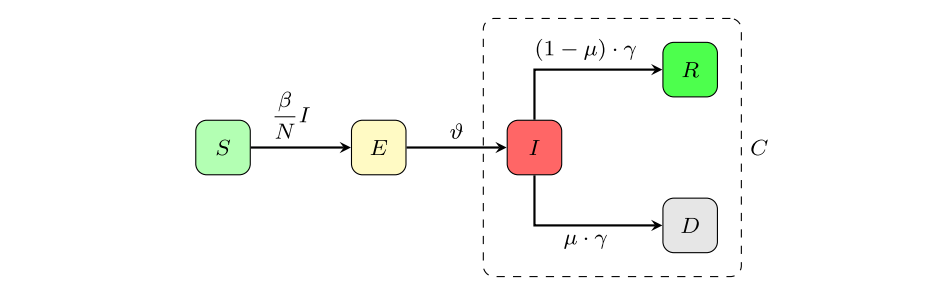
\includegraphics[scale = 0.6]{figTomas.png}
    \caption{Diagrama representando o modelo SEIR proposto em \cite{goetz2020covid}.}
\end{center}
\end{figure}

No diagrama proposto, $S$ representa a classe dos Suscetíveis, $E$ dos Expostos, $I$ dos Infectados, $R$ dos Recuperados e $D$ dos Mortos. Quanto aos parâmetros indicados, $\beta$ representa a taxa de contágio, $\vartheta$ o período de incubação, $\gamma$ a taxa de recuperação e $\mu$ a mortalidade. 

Os suscetíveis são os indivíduos da população que ainda não foram infectados. Após serem infectados eles se tornam expostos e com uma taxa $\vartheta$ se tornam infecciosos, quando infecciosos eles infectam os suscetíveis com uma probabilidade $\beta$ e se tornam recuperados com uma taxa $\gamma$, ou mortos com uma taxa de mortalidade $\mu$.
O compartimento C representa todos os indíviduos infectados em qualquer estágio, esse compartimento foi criado para auxiliar na comparação dos dados do modelo com os dados reais. 

\noindent Matematicamente, esse modelo pode ser expresso por:
\begin{center}
$$
\begin{cases}
\dot S = -\cfrac{\beta S I}{N} \hspace{2.75cm} S(t_0)= N - E_0 - I_0\\
\dot E = \cfrac{\beta S I}{N} \hspace{3.0cm} E(t_0) = E_0\\
\dot I = \vartheta E - \gamma I \hspace{2.35cm} I(t_0) = I_0\\
\dot R = (1- \mu) \cdot \gamma I\hspace{1.7cm} R(t_0) = 0 \\
\dot D = \mu \cdot \gamma I \hspace{2.7cm}  D(t_0) = 0
\end{cases}
$$
\end{center}

O $t_0$ considerado foi 1º de março, data em que a Alemanha atingia mais de 100 casos confirmados. Como a primeira morte foi reportada em 09 de março, o número de mortos inicial foi assumido como zero. O número de recuperados foi considerado insignificante pelo autor, por essa razão foi considerado nulo. 

No modelo acima o valor de $\beta$ foi considerado contante, porém sabemos que isso não é condizente com a realidade, visto que as medidas de combate ao espalhamento da COVID-19 atuam diminuindo o valor de $\beta$. Assim, para incluir essas medidas adotadas pelo governo, o autor propôs um novo modelo, com a taxa de contágio $\beta (t)$ definida em função do tempo como uma função por partes. 

Na Alemanha, em 16 de Março, as escolas, jardins de infância e universidades foram fechados, e em 22 de março medidas de distanciamento social foram impostas na Alemanha, com o intuito de diminuir o valor do $\beta$. Assim, a função $\beta(t)$ é expressa por:
\begin{center}
$$
\beta(t) = 
\begin{cases}
\beta_0 : \text{t $<$ 16 de Março} \\
\beta_1 : \text{16 de Março $<$ t $<$ 22 Março} \\
\beta_2 : \text{t $>$ 22 de Março}
\end{cases}
$$
\end{center}

Assim, o novo modelo é expresso por

\begin{center}
$$
\begin{cases}
\dot S = -\cfrac{\beta (t) S I}{N} \hspace{2.3cm} S(t_0)= N - E_0 - I_0\\
\dot E = \cfrac{\beta (t) S I}{N} \hspace{2.5cm} E(t_0) = E_0\\
\dot I = \vartheta E - \gamma I \hspace{2.35cm} I(t_0) = I_0\\
\dot R = (1- \mu) \cdot \gamma I\hspace{1.7cm} R(t_0) = 0 \\
\dot D = \mu \cdot \gamma I \hspace{2.7cm}  D(t_0) = 0
\end{cases}
$$
\end{center}

\noindent Veja que se $\beta := \beta_0 = \beta_1 = \beta_2$ temos o modelo anterior.

Além disso, segundo o Robert Koch Institute \cite{RKI} há uma diferença de 10 dias entre o início dos sintomas e a entrada em uma unidade de terapia intensiva. Pensando nessa diferença de tempo, o autor propôs um novo modelo incorporando uma diferença de tempo, $\tau = 14$ dias, entre os primeiros sintomas e a morte. Sendo o novo modelo expresso por:
\begin{center}
$$
\begin{cases}
\dot S = -\cfrac{\beta (t) S I}{N} \hspace{4.8cm} S(t_0)= N - E_0 - I_0\\
\dot E = \cfrac{\beta (t) S I}{N} \hspace{5.0cm} E(t_0) = E_0\\
\dot I = \vartheta E - \gamma [(1 - \mu)I + \mu I(t - \tau)] \hspace{1.2cm} I(t_0) = I_0\\
\dot R = (1- \mu) \cdot \gamma I\hspace{4.2cm} R(t_0) = 0 \\
\dot D = \mu \cdot \gamma I(t - \tau) \hspace{4.0cm}  D(t_0) = 0
\end{cases}
$$
\end{center}

Para resolver a equação diferencial com retardo é necessário uma "história" inicial para o compartimento dos infectados.
Nos três modelos foram assumidos $\vartheta = 1/2$ e $\gamma = 1/10$, assim, são assumidos fixos e constantes um período de incubação de 2 dias e um período de recuperação de 10 dias, sendo os outros parâmetros do modelo fitados.



\subsection{Meso-scale modeling of COVID-19 spatio-temporal outbreak dynamics in Germany}

O artigo \cite{kergassner2020meso} propõe um modelo SIQRD espacial que inclui as políticas locais adotadas para predizer a evolução espacial-temporal da pandemia na Alemanha. O diagrama da Figura 2 descreve o modelo básico adotado, a partir do qual é incluida a interação entre diferentes regiões. 

O modelo proposto divide a população em 5 classes, Suscetíveis, aqueles que ainda não foram infectados pela doença representados por S, infectados, representados por I, que representa os indivíduos que estão com o vírus e estão infectando outras pessoas. O modelo considera que uma porção dos infectados são indentificados e são quarentenados, representados pela letra Q. Os indivíduos que permancem em I, são considerados os indivíduos que tem sintomas mais leves da doença, ou não possuem sintomas, logo, eles se recuperam e vão para caixa R. Quanto aos indivíduos quarentenados, eles são os indivíduos com sintomas mais graves, assim, possuem duas possibilidades eles podem se recuperar e ir para R, ou vir a óbito e ir para D, que representa os óbitos. O modelo não inclui uma classe para os expostos, visto que o principal objetivo é analisar a diferença entre os indivíduos sintomáticos e assintomáticos e seu impacto na dinâmica de espalhamento da doença.

\begin{figure}[h]
\begin{center}
    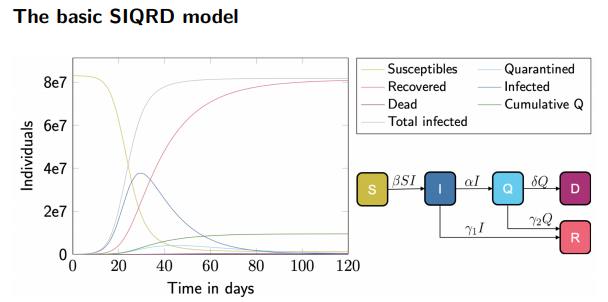
\includegraphics[scale = 0.6]{diag-meso.png}
    \caption{Diagrama representando o modelo básico SIQRD proposto em \cite{kergassner2020meso}.}
\end{center}
\end{figure}

\noindent O modelo é definido pelo seguinte sistema de equações diferenciais ordinárias:

\begin{center}
$$
\begin{cases}
\dot S = \beta S I \\
\dot I = \beta S I - \alpha I - \gamma_1 I\\
\dot Q = \alpha I - \gamma_2 Q - \delta Q\\
\dot R = \gamma_1 I + \gamma_2 Q \\
\dot D = \delta Q
\end{cases}
$$
\end{center}

O sistema assume a população normalizada, assim $S + I + Q +R + D = 1$, logo $\dot S + \dot I + \dot Q +\dot R + \dot D = 0$. No tocante aos parâmetros do modelo, $\beta$ representa a taxa de contágio, $\alpha$ o tempo entre um indivíduo ser infectado, testado e colocado em quarentena. Além disso, $\gamma_1$ representa a taxa de recuperação dos indivíduos infectados assintomáticos ou com poucos sintomas, $\gamma_2$ a taxa de recuperação dos individuos que são quarentenados e $\delta$ a taxa de mortalidade dos indivíduos quarentenados.

Além disso, o autor faz o uso de uma expressão para a subnotificação, $\omega$ e a mortalidade real, $\mu$, a partir dos parâmetros. As expressões utilizadas são:
$$\omega = 1 + \cfrac{\gamma_1}{\alpha}$$
$$\mu = \cfrac{\delta}{\gamma_2 + \delta} \cfrac{\alpha}{\alpha + \gamma_1}$$


Ademais, no artigo ele adota a seguinte expressão para o cálculo do número de reprodução efetivo da doença, definido como a razão entre a razão entre a taxa de entrada e de saída do compartimento $I$:
$$R_{eff}(t) = \cfrac{\beta(t)S(t) (\omega -1)}{\omega \gamma_1} \geq \cfrac{\beta(t) (\omega -1)}{\omega \gamma_1} = R_0(t)$$

No início da epidemia, grande parte da população é suscetível, assim, podemos assumir $S(t) =1$. A partir da expressão acima fica evidente a relação da subnotificação com os valor do $R_{eff}(t)$. O autor do artigo discute também a importância de considerar que $\alpha$ e $\omega$ variam no decorrer do tempo, para melhor compreender a dinâmica do processo.


O autor faz uma adaptação deste modelo para torná-lo espacial, considerando a influência do fluxo entre diferentes regiões da Alemanha no espalhamento da doença. No entanto, como não irei utilizar um modelo espacial, não considerei relevante incluir a metodologia adotada pelo autor nesse caso.

\subsection{Predicting the number of reported and unreported cases for the COVID-19 epidemics in China, South Korea, Italy, France, Germany and United Kingdom}

O artigo \cite{liu2020predicting} propõe um sistema de equações diferenciais ordinárias para modelar o espalhamento do COVID-19 em 6 países diferentes, entre eles a Alemanha. O modelo proposto divide a população em 4 classes diferentes, Suscetíves, representados pela letra $S$, assintomáticos (com poucos ou nenhum sintomas), representados por $I$, casos sintomáticos reportados representados por $R$ e casos sintomáticos não reportados (com poucos sintomas), representados por $U$. 

O modelo proposto não assume um périodo de latência para doença, visto que, os autores deram maior significado ao impacto dos indivíduos assintomáticos (com poucos ou nehum sintoma) no espalhamento da doença. Esse mesmo modelo com a inclusão da classe dos expostos, foi proposto pelos mesmos autores desse artigo em \cite{liu2020covid}. Na Figura 3 há um diagrama representando o modelo.
\begin{figure}[h]
\begin{center}
    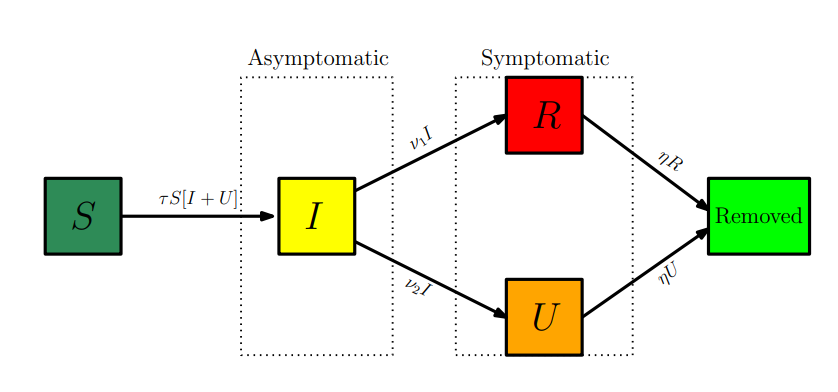
\includegraphics[scale = 0.6]{diag-Liu.png}
    \caption{Diagrama representando o modelo proposto em \cite{liu2020predicting}.}
\end{center}
\end{figure}

O sistema de equações que define o modelo está definido abaixo, vale ressaltar que ele considera que os indivíduos assintomáticos ($I$) e os indivíduos sintomáticos não reportados ($U$) podem transmitir o vírus. Isso se dá em função do fato de que os indivíduos reportados são quarentenados.
\begin{center}
$$
    \begin{cases}
    \dot S(t) = \tau(t)S(t)[I(t) + U(t)],\\
    \dot I(t) = \tau(t)S(t)[I(t) + U(t)] - \nu I(t),\\
    \dot R(t) = \nu_1I(t) - \eta R(t),\\
    \dot U(t) = \nu_2I(t) - \eta U(t)
    \end{cases}
$$
\end{center}
Com condições iniciais: 
$$S(t_1) = S_1>0, I(t_1) = I_1>0, R(t_1) = R_1 \leq 0 \text{ e } U(t_0) = U_1 \leq 0.$$

A taxa de transmissão $\tau(t)$, varia no decorrer do tempo. No início da epidemia ela é constante. Porém com as medidas públicas de combate ao espalhamento no vírus, como fechamento de escolas, uso de máscaras, política de distanciamento social ela tende a diminuir. Nesse sentido, os autores assumiram que essa diminuição ocorre como um decrescimento exponencial. Matematicamente, $\tau(t)$ é expressa por:
\begin{center}
$$
     \tau(t) =
    \begin{cases}
    \tau_1, 0 \geq t \geq N,\\
    \tau_1 exp(-\mu(t-N)), t > N.
    \end{cases}
$$
\end{center}
Onde $N$ representa a data que as intervenções adotadas se tornaram efetivas e $\mu$ quantifica a intensidade dessas medidas.

Os outros parâmetros do modelo, presentes no sistema de equações estão representados na tabela abaixo. 

\begin{table}[h]
\centering
\begin{small}
\caption{Parâmetros e condições iniciais do modelo} \label{Tabela1}
\begin{tabular}{|p{2.5cm}|p{10.5cm}|p{2cm}|}
\hline
Símbolo & Interpretação & Método\\
\hline
$t_0$ & Data de início da epidemia & Ajustado \\
\hline
$S_0$ & Número de suscetíveis no tempo $t_0$ & Fixo\\
\hline
$I_0$ & Número de infectados assintomáticos no tempo $t_0$ & Ajustado\\
\hline
$R_0$ & Número de indivíduos infectados reportados no tempo $t_0$ & Ajustado \\
\hline
$U_0$ & Número de indivíduos infectados não reportados no tempo $t_0$ & Ajustado \\
\hline
$\tau(t)$ & Taxa de transmissão no tempo t & Ajustado \\
\hline
$N$ & Data em que as intervenções públicas se tornaram efetivas & Ajustado \\
\hline
$\mu$ & Intensidade das medidas de intervenção públicas adotadas & Ajustado \\
\hline
$1/\nu$ & Tempo médio durante um infectado assintomático é assintomático & Fixo \\
\hline
$f$ & Fração dos infectados assintomáticos que são reportados & Fixo \\
\hline
$\nu_1  = \nu f$ & Taxa com que os assintomáticos infectados se tornam assintomáticos reportados & Ajustado \\
\hline
$\nu_2 = (1-f)\nu$ & Taxa que os infectados assintomáticos se tornam infectados sintomáticos não reportados & Ajustado \\
\hline
$1 / \nu$ & Tempo médio em que os infectados sintomáticos possuem sintomas & Fixo\\
\hline
\end{tabular}
\end{small}
\end{table}

\noindent O número acumulado de casos reportados no tempo (t) é obtido por:
$$\dot{CR}(t) = \nu_1I(t)$$
E o número acumulado de casos não reportados por:
$$\dot{CU}(t) = \nu_2 I(t)$$

 
%%%%%%%%%%%%%%%%%%%%%%%%%%%%%%%%%%%%%%%%%%%%%%%%%%%%%%%%%%%%%%
\section{Metodologia}
\subsection{Obtenção dos dados}

Os dados utilizados nesse trabalho foram retirados da plataforma \url{https://ourworldindata.org/}. Para capturar os dados foi criado um script em python disponível em \url{https://github.com/eduardocorrearaujo/Avaliacoes-MM4-/blob/master/Dados_Alemanha.ipynb}.

Utilizando os dados disponíveis, foi possível plotar os gráficos abaixo. A Figura 4 representa os casos diários e acumulados na Alemanha, a partir do gráfico fica claro que os casos começaram a se estabilizar, porém continuaram a subir indicando uma segunda onda.

Em comparativo, a Figura 5 representa os óbitos diários e acumulados, a partir do gráfico podemos observar que o número de mortos não aumentaram seguindo o mesmo crescimento do número de casos. Isso indica uma diferença na mortalidade da doença, a qual como dita acima está relacionada com o fato, que de grande parte dos infectados nessa segunda onda fazem parte da parcela mais jovem da população, que normalmente, tem sintomas mais leves da doença. Esse fator é muito importante para a modelagem do fenômeno.

\begin{figure}[h]

\center
\subfigure{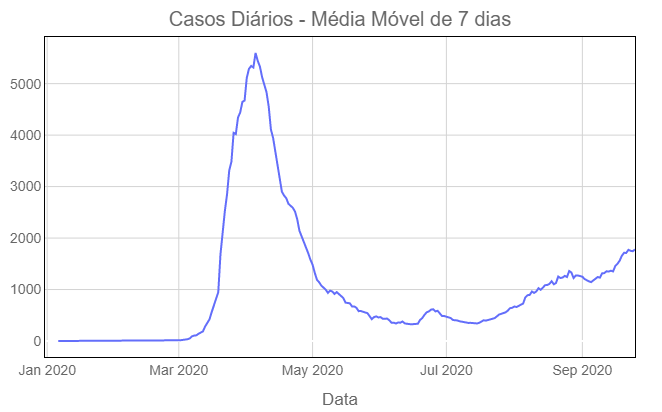
\includegraphics[width=8.3cm]{casos_diarios.png}}
\qquad
\subfigure{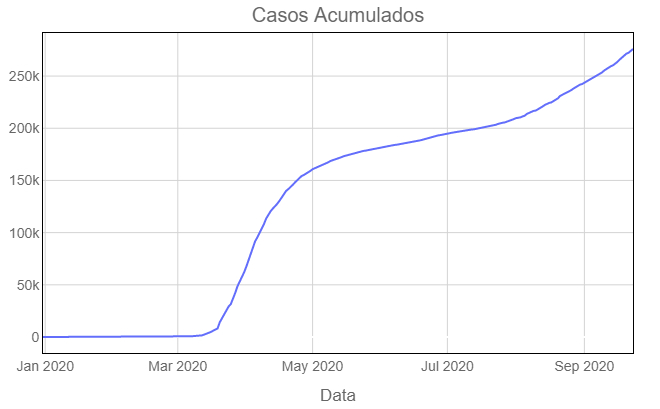
\includegraphics[width=8.3cm]{casos_acumulados.png}}
\caption{O gráfico do lado esquerdo representa os casos diários suavizados por média móvel de 7 dias e o gráfico do lado direito representa os casos acumulados.}

\end{figure}

\begin{figure}[h]

\center
\subfigure
{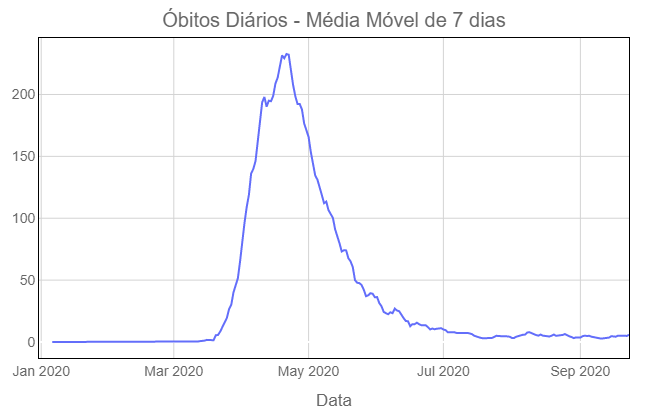
\includegraphics[width=8.3cm]{obitos_diarios.png}}
\qquad
\subfigure
{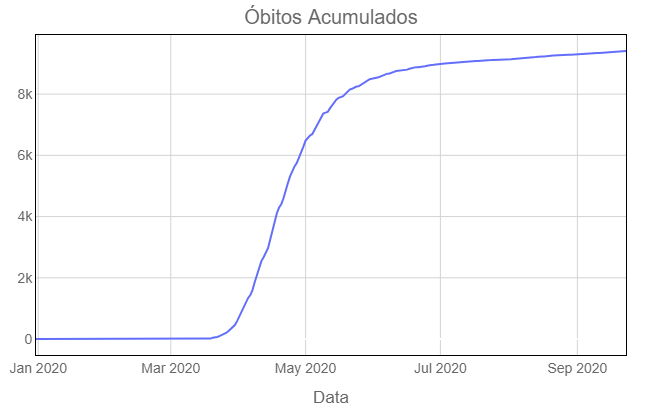
\includegraphics[width=8.3cm]{obitos_acumulados.png}}
\caption{O gráfico do lado esquerdo representa os óbitos diários suavizados por média móvel de 7 dias e o gráfico do lado direito representa os óbitos acumulados.}

\end{figure}

\newpage
\subsection{Modelo SEIASRD}
Nesse trabalho é proposto um modelo extendido do tipo SEIR para analisar a dinâmica do espalhamento da COVID-19 na Alemanha.

O modelo adotado  divide a população em 7 classes diferentes: $S$ representa os indivíduos suscetíveis que ainda não foram infectados, $E$ representa os indivíduos expostos, que estão no período de incubação, já que há conhecimento clínico de que a doença possui um período de incubação. Esses indivíduos são aqueles que foram infectados, mas ainda não desenvolveram nenhum sintoma e não estão infecciosos. Passado o período de incubação,   o modelo assume duas possibilidades distintas: o indivíduo pode ir para $Ia$ que engloba os indivíduos assintomáticos, com poucos sintomas que não vão para as estatísticas ou para $Is$ que engloba os indivíduos com sintomas mais graves que são reportados. Se o indivíduo for assintomático ele se recupera indo para $Ra$ e se for sintomático pode se recuperar indo para $Rs$ ou acabar falecendo indo  para $D$ que engloba os óbitos.

Além disso, no modelo é considerado que os indivíduos sintomáticos são identificados e quarentenados, assim, o modelo considera um fator de correção $q$ para a sua infectividade, visto que como grande parte dos infectados são quarentenados eles não tem o mesmo potencial de infectar outros indivíduos como os indivíduos assintomáticos. Achei relevante colocá-los, visto que, normalmente, há uma diferença entre início dos sintomas e a identificação e  quarentena dos casos e nesse período esses indivíduos podem infectar outras pessoas. Foi feita a divisão entre assintomáticos e sintomáticos, visto que como os primeiros não tem sintomas graves, na grande maior parte dos casos não são identificados e isolados, assim, acabam tendo contato com um número muito maior de pessoas, o que por sua vez implica que eles infectem um número maior de pessoas. Veja na Figura 6 o diagrama do modelo e na Tabela 2 o significado de cada um dos parâmetros apresentados no diagrama.

\begin{figure*}[h!]
    \centering
    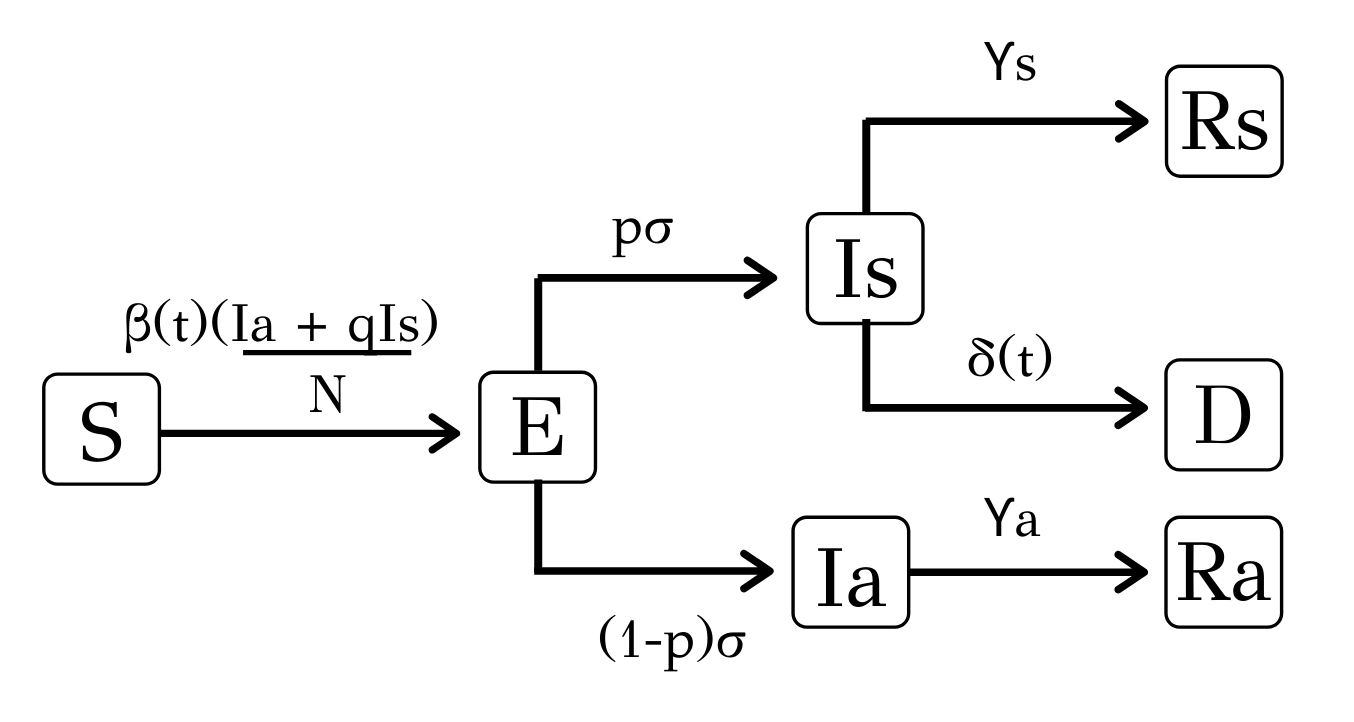
\includegraphics[scale = 0.35]{Diagrama Modelo.png}
    \caption{Diagrama do modelo SEIASRD - SEIR extendido.}
\end{figure*}


O modelo é definido pelo seguinte sistema de Equações Diferenciais Ordinárias:

\begin{center}
$$
\begin{cases}
\dot S = \cfrac{-\beta(t)S(Ia + qIs)}{N} \\
\dot E = \cfrac{\beta(t)S(Ia + qIs)}{N} - \sigma E \\
\dot {Ia} = p\sigma E - \gamma_aIa\\
\dot {Is} = (1-p)\sigma E - \gamma_sIs - \cfrac{\gamma_S \delta (t)Is}{1 - \delta(t)}\\
\dot {Ra} = \gamma_aIa\\
\dot {Rs} = \gamma_sIs\\
\dot {D} = \cfrac{\gamma_S \delta (t)Is}{1 - \delta(t)}

\end{cases}
$$
\end{center}

\noindent Com condições iniciais $$S(t_0) = S_0 > 0, E(t_0) = E_0 \geq 0, Ia(t_0) = Ia_0 >0, Is(t_0) = Is_0 \geq 0$$
$$Ra(t_0) = Ra_0 \geq 0, Rs(t_0) = Rs_0 \geq 0, D(t_0) = D_0 \geq 0.$$ Esse modelo possui a propriedade de conservação da massa, sendo assim, $S + E + Ia + Is + Ra + Rs + D = N$, ou seja, a população é sempre constante, o modelo não considera efeitos de imigração, emigração, natalidade e mortalidade, é considerada apenas a mortalidade da doença.

\begin{table}[h]
\centering
\begin{small}
\caption{Parâmetros do modelo} \label{Tabela1}
\begin{tabular}{|p{2cm}|p{14cm}|}
\hline
            Parâmetro & Significado \\
\hline
$t_0$ & tempo inicial \\
\hline
$S_0$ & Número de indivíduos suscetíveis em $t_0$\\
\hline 
$E_0$ & Número de indivíduos expostos em $t_0$\\
\hline 
$Ia_0$ & Número de indivíduos assintomáticos (com poucos ou nenhum sintoma) em $t_0$\\
\hline 
$Ia_0$ & Número de indivíduos sintomáticos em $t_0$\\
\hline 
$Ra_0$ & Número de indivíduos recuperados assintomáticos em $t_0$\\
\hline 
$Rs_0$ & Número de indivíduos recuperados sintomáticos em $t_0$\\
\hline 
$D_0$ & Número de indivíduos mortos em $t_0$\\
\hline 
$\beta(t)$ & Taxa de contágio, no modelo é representada por uma função degrau dependente do tempo. \\
\hline
$q$ & Correção para a infectividade dos indivíduos sintomáticos, isso é feito em virtude do protocolo de quarentena para esses indivíduos o que diminui sua probabilidade de infectar outras pessoas.\\
\hline
$N$ & População da Alemanha. \\
\hline
$\sigma$ & $1/ \sigma$ representa o tempo de incubação do vírus. \\
\hline
$p$ & Porcentagem dos indivíduos expostos que se tornam assintomáticos.\\
\hline
$\gamma_a$ & $1 / \gamma_a$ representa o tempo de recuperação dos indivíduos assintomáticos. \\
\hline
$\gamma_s$ & $1 / \gamma_s$ representa o tempo de recuperação dos indivíduos sintomáticos.\\
\hline
$\delta(t)$ & taxa de mortalidade da doença, que é expressa por uma funçaõ degrau dependente do tempo. \\
\hline
\end{tabular}
\end{small}
\end{table}

A taxa de contágio, $\beta(t)$ foi considerada variável para incluir no modelo as políticas adotadas em relação a epidemia, assim como feito em \cite{goetz2020covid}, as quais estão representas da tabela 1. Assim:

\begin{center}
$$
\beta(t) = 
\begin{cases}
\beta_0 : \text{t $<$ 16 de Março} \\
\beta_1 : \text{16 de Março $<$ t $<$ 22 Março} \\
\beta_2 : \text{22 de Março $<$ t $<$ 20 de Abril}\\
\beta_3 : \text{20 de Abril $<$ t $<$ 06 de Maio} \\
\beta_4 : \text{06 de Maio $<$ t $<$ 15 de Junho} \\
\beta_5 : \text{15 de Junho $<$ t $<$ 01 de Agosto}\\
\beta_6: \text{ t $>$ 01 de Agosto}\\
\end{cases}
$$
\end{center}

\noindent Note que se $\beta_0 = \beta_1 = \beta_2 =\beta_3 =\beta_4 =
\beta_5 = \beta_6$ temos o modelo com $\beta$ constante. Veja um exemplo do comportamento dessa função na Figura 7.

\begin{figure}[h]
\begin{center}
    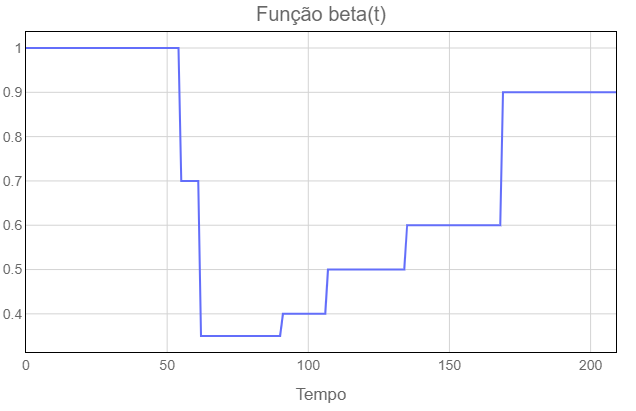
\includegraphics[scale = 0.5]{beta(t).png}
    \caption{Função beta(t) considerando $b_0 = 1.0, b_1 = 0.7, b_2 = 0.35, b_3 = 0.4, b_4 = 0.5, b_5 = 0.6, b_6 = 0.9$.}
\end{center}
\end{figure}


Para a taxa de mortalidade será considerada uma taxa de mortalidade variável no decorrer do tempo. É adotada essa postura, pois a mortalidade da doença, nesse caso é influenciada por três grandes fatores:
\begin{enumerate}
    \item Aumento do número de testes.
    \item Aumento do conhecimento médico sobre a melhor forma de tratar a doença.
    \item Diferença na idade dos infectados. A segunda onda da epidemia na Alemanha tem como característica que a maior parte dos infectados fazem parte da parcela mais jovem da população, que tem uma mortalidade menor.
\end{enumerate}
Por esses motivos foi adotado um decrescimento exponencial para a mortalidade no decorrer do tempo. Assim, 
\begin{center}
$$
\delta(t) = 
    \begin{cases}
    \delta_0: \text{ 0  $\leq t \leq $ d }\\
    \delta_0 e^{-\mu (t - d)}: \text{t $>$ d}
    \end{cases}
$$
\end{center}
Onde $\delta_0$ representa o valor inicial para a mortalidade, $d$ representa a data em que a mortalidade começou a diminuir e $\mu$ a intensidade desse decrescimento. Veja abaixo um exemplo do comportamento dessa função na Figura 8.

\begin{figure}[h]
\begin{center}
    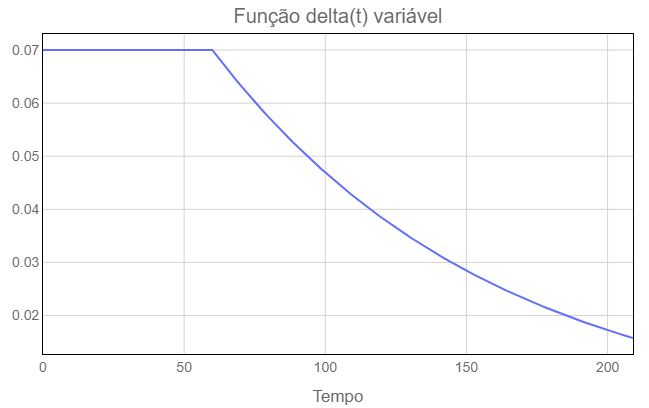
\includegraphics[scale = 0.5]{delta(t).png}
    \caption{Função $\delta(t)$ considerando $\delta_0 = 0.07, \mu = -0.01, d = 60$.}
\end{center}
\end{figure}
Veja na Figura 9 uma solução númerica do modelo SEIASRD com as seguintes condições:
$$N = 83.2 \cdot 10^6, S_0 = N - 1, E_0 = 0,Ia_0 = 1, Is_0 = 0, Ra_0 = 0, Rs = 0, D = 0,$$
$$ q = 0.2, p = 0.4, \sigma = 1/5, \gamma_a = 1/9, \gamma_s = 1/15 $$
Os valores de $\beta(t)$ e $\delta(t)$ são os mesmos assumidos para gerar as Figuras 7 e 8.


\begin{figure}[h]
\begin{center}
    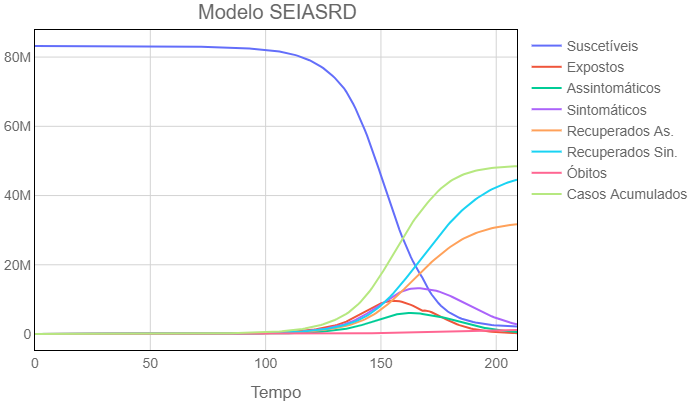
\includegraphics[scale = 0.6]{SEIASRD.png}
    \caption{Diagrama representando a solução numérica do  modelo SEIASRD proposto.}
\end{center}
\end{figure}



\noindent O código responsável por gerar essas imagens está disponível em: 

\noindent \url{https://github.com/eduardocorrearaujo/Avaliacoes-MM4-/blob/master/SEIASRD.ipynb}.

 
\newpage
\subsubsection{Análise Dimensional do Modelo}
Como visto anteriormente, o modelo é definido pelo seguinte sistema de equações diferenciais ordinárias:
\begin{center}
$$
\begin{cases}
\dot S = \cfrac{-\beta(t)S(Ia + qIs)}{N} \\
\dot E = \cfrac{\beta(t)S(Ia + qIs)}{N} - \sigma E \\
\dot {Ia} = p\sigma E - \gamma_aIa\\
\dot {Is} = (1-p)\sigma E - \gamma_sIs - \cfrac{\gamma_S \delta (t)Is}{1 - \delta(t)}\\
\dot {Ra} = \gamma_aIa\\
\dot {Rs} = \gamma_sIs\\
\dot {D} = \cfrac{\gamma_S \delta (t)Is}{1 - \delta(t)}

\end{cases}
$$
\end{center}


Vamos assumir que a escala de tempo, $t$ do modelo é expressa em dias. Sabemos que os lados esquerdos das equações acima tem dimensão $[M]/[T]$, onde $M$ representa a massa e $T$ o tempo. Assim, na primeira equação concluímos que $S, I_a, E, N$ tem dimensão $[M]$, $\beta(t)$ tem dimensão $[T]^{-1}$ e $q$ é adimensional. Na segunda equação, concluí-se que $\sigma$ tem dimensão $[T]^{-1}$. Na terceira equação concluí-se que $\gamma_a$ tem dimensão $[T]^{-1}$ e $p$ é adimensional. Na quarta equação concluí-se que $\gamma_s$ tem dimensão $[T]^{-1}$ e $\delta(t)$ é adimensional. 

Para tornar o sistema adimensional, primeiro no tocante a massa, podemos assumir que 

$S^* = \cfrac{S}{N}$, logo $S^*$ é adimensional, derivando ambos os lados em relação ao tempo, encontramos:
$$\cfrac{dS^*}{dt} = \cfrac{dS}{dt} \cdot \cfrac{1}{N} = \cfrac{-\beta(t)S(Ia + qIs)}{N \cdot N}$$
Procedendo do mesmo modo com as outras equações, encontramos que:
$$E^* = \cfrac{E}{N} \implies \cfrac{dE^*}{dt} = \cfrac{dE}{dt} \cdot \cfrac{1}{N} = \cfrac{\beta(t)S(Ia + qIs)}{N \cdot N} - \cfrac{\sigma E}{N}$$
$$Ia^* = \cfrac{Ia}{N} \implies \cfrac{dIa^*}{dt} = \cfrac{dIa}{dt} \cdot \cfrac{1}{N} = \cfrac{ p\sigma E - \gamma_aIa}{N}$$
$$Is^* = \cfrac{Is}{N} \implies \cfrac{dIs^*}{dt} = \cfrac{dIs}{dt} \cdot \cfrac{1}{N} = \cfrac{ (1-p)\sigma E - \gamma_sIs - \cfrac{\gamma_S \delta (t)Is}{1 - \delta(t)}}{N}$$
$$Ra^* = \cfrac{Ra}{N} \implies \cfrac{dRa^*}{dt} = \cfrac{dRa}{dt} \cdot \cfrac{1}{N} = \cfrac{\gamma_aIa}{N}$$
$$Rs^* = \cfrac{Rs}{N} \implies \cfrac{Rs^*}{dt} = \cfrac{dRs}{dt} \cdot \cfrac{1}{N} = \cfrac{\gamma_aIs}{N}$$
$$D^* = \cfrac{D}{N} \implies \cfrac{dD^*}{dt} = \cfrac{dD}{dt} \cdot \cfrac{1}{N} = \cfrac{\gamma_S \delta (t)Is}{N(1 - \delta(t))}$$



Substituindo $ S^* = \cfrac{S}{N}, E^* = \cfrac{E}{N}, Ia^* = \cfrac{Ia}{N},Is^* = \cfrac{Is}{N},Ra^* = \cfrac{Ra}{N},Rs^* = \cfrac{Rs}{N},D^* = \cfrac{D}{N} $ nas equações que encontramos para $\dot S^*,\dot E^*,\dot Ia^*,\dot Is^*,\dot Ra^*, \dot Rs^*, \dot D^*$, o modelo adimensional no tocante a massa é:
\begin{center}
$$
\begin{cases}
\dot S^* = -\beta(t)S^*(Ia^* + qIs^*) \\
\dot E^* = \beta(t)S^*(Ia^* + qIs^*) - \sigma E^* \\
\dot {Ia^*} = p\sigma E^* - \gamma_aIa^*\\
\dot {Is^*} = (1-p)\sigma E^* - \gamma_sIs^* - \cfrac{\gamma_S \delta (t)Is^*}{1 - \delta(t)}\\
\dot {Ra^*} = \gamma_aIa^*\\
\dot {Rs^*} = \gamma_sIs^*\\
\dot {D^*} = \cfrac{\gamma_s \delta (t)Is^*}{1 - \delta(t)}

\end{cases}
$$
\end{center}

\noindent onde $S^* + E^* +Ia^*+I^*s+R^*a+R^*s+D^* = \cfrac{N}{N} = 1$

Resta agora adimensionalizar em relação ao tempo. Se $t^* = \gamma_a t$, note que $t^*$ é adimensional. Derivando ambos os lados em relação a $t^*$ encontramos:
$$t^* = \gamma_a t \implies \cfrac{dt^*}{dt^*} = \gamma_a \cfrac{dt}{dt^*} \implies \cfrac{dt}{dt^*} = \cfrac{1}{\gamma_a}$$

Para a primeira equação do sistema adimensional em relação a massa, aplicando a regra da cadeia, temos que:
$$\cfrac{dS^*}{dt^*} = \cfrac{dS^*}{dt} \cdot  \cfrac{dt}{dt^*} = -\beta(t)S^*(Ia^* + qIs^*) \cdot \cfrac{1}{\gamma_a}$$

Aplicando a mesma análise para cada uma das outras equações do sistema obtemos o seguinte sistema adimensional:

\begin{center}
$$
\begin{cases}
\cfrac{dS^*}{dt^*} = \cfrac{-\beta(t)S^*(Ia^* + qIs^*)}{\gamma_a} \\
\cfrac{dE^*}{dt^*}  = \cfrac{\beta(t)S^*(Ia^* + qIs^*) - \sigma E^* }{\gamma_a}\\
\cfrac{dIa^*}{dt^*}  = \cfrac{p\sigma E^* - \gamma_aIa^*}{\gamma_a}\\
\cfrac{dIs^*}{dt^*}  = \cfrac{(1-p)\sigma E^* - \gamma_sIs^*}{\gamma_a} - \cfrac{\gamma_S \delta (t)Is^*}{\gamma_a(1 - \delta(t))}\\
\cfrac{dRa^*}{dt^*}  = Ia^*\\
\cfrac{dRs^*}{dt^*}  = \cfrac{\gamma_sIs^*}{\gamma_a}\\
\cfrac{dD^*}{dt^*}  = \cfrac{\gamma_s \delta (t)Is^*}{\gamma_a(1 - \delta(t))}

\end{cases}
$$
\end{center}

\bibliographystyle{abbrv}
\bibliography{ref}

\end{document}
